%----------------------------------------------------------------------------------------
%	The Perceptron CHAPTER 
%----------------------------------------------------------------------------------------
\chapterimage{ChapterCover.pdf} % Chapter heading image
\chapter{The Perceptron}

\epigraph{\textit{Artificial intelligence is the science of making machines do things that would require intelligence if done by men.}}{\rightline{{\rm --- \href{https://en.wikipedia.org/wiki/Marvin_Minsky}{Marvin Minsky}}}}

\minitoc
\newpage
\section{Introduction to the Perceptron}
\subsection{Historical Significance}
The perceptron is a fundamental building block in artificial neural networks, serving as a simplified model of a biological neuron. Introduced by American psychologist Frank Rosenblatt (1928 – 1971) in 1958, the perceptron is designed to perform binary classification by making a decision based on weighted inputs. It consists of input connections, each associated with a weight, a summation function, and an activation function. The perceptron receives multiple input signals, multiplies each by its corresponding weight, sums these products, and then passes the result through an activation function to produce an output. This output is typically binary, mimicking the all-or-nothing firing of a biological neuron. The perceptron's ability to learn comes from adjusting its weights based on the error between its output and the desired output, allowing it to improve its classification performance over time. While limited in its capacity to solve complex problems on its own, the perceptron laid the groundwork for more sophisticated neural network architectures and played a crucial role in the development of machine learning and artificial intelligence.

\subsection{Biological Relevance}
Neurons share several key mechanisms that make them function similarly to a perceptron, the basic computational unit in artificial neural networks. Both aggregate multiple inputs, summing them to determine if they exceed a threshold. Neurons receive inputs from other neurons via dendrites. These inputs are chemical signals called neurotransmitters, which cause changes in the electrical potential of the neuron's membrane (excitatory or inhibitory post-synaptic potentials). The perceptron takes numerical inputs, which are weighted sums of features or previous layer outputs. 
The perceptron’s weights are numerical values assigned to inputs, determining their importance in the perceptron’s computation and these can be adjusted (during “learning”) to optimize performance. Similarly, synapses on neurons vary in strength based on factors like neurotransmitter release and receptor sensitivity, influencing the impact of each input. Synaptic plasticity (e.g., long-term potentiation) adjusts these weights over time based on experience.

Both the neuron and the perceptron perform an integration process to evaluate the overall ``input signal strength." The neuron integrates all incoming signals (excitatory and inhibitory) at the axon hillock, calculating the net membrane potential, which determines whether or not an action potential will be generated. The perceptron applies a step or non-linear activation function (e.g., sigmoid, ReLU) to the weighted sum to determine the output.
	
The neuron and the perceptron can also both pass a processed signal forward to influence subsequent units in the network. The perceptron sends its output to other perceptrons or layers in a network.  The action potential travels down the axon and triggers the release of neurotransmitters at synapses, which communicate with other neurons or effector cells.
	
Finally, both neurons and perceptrons refine their connections and processing capabilities over time to improve performance or adapt to changing environments. Neurons adapt through mechanisms like Hebbian learning ("cells that fire together, wire together"), strengthening or weakening synaptic connections based on activity patterns. Perceptrons learn by adjusting weights using algorithms like gradient descent, minimizing error signals based on feedback.

While neurons and perceptrons share fundamental similarities, such as input integration, weighted summation, and threshold-based activation, neurons are far more complex in structure and function. A biological neuron operates within a dynamic, adaptive network influenced by time, space, and chemical signaling. Unlike the simple numerical inputs and weights of a perceptron, neurons process inputs through complex interactions of excitatory and inhibitory neurotransmitters, with synaptic strengths modulated by activity patterns over time. These processes allow neurons to exhibit temporal dynamics, such as short-term memory and firing rate adaptation, which add layers of functionality beyond the capabilities of a standard perception.

Additionally, neurons interact through intricate networks with feedback loops, diverse neurotransmitter systems, and modulatory effects that influence signal propagation. While perceptrons rely on static activation functions like step or ReLU, neurons display non-linear behaviors, such as burst firing, oscillations, and long-term plasticity, allowing for richer and more flexible processing. Neural circuits are not just reactive but adaptive, with mechanisms like Hebbian learning and synaptic plasticity enabling them to restructure and optimize their connections in response to experience. These differences highlight the biological sophistication of neurons compared to the simplified, idealized model of the perception.

\subsection{Significance in machine learning and AI development}

\begin{wrapfigure}{R}{0.4\textwidth}
\begin{tcolorbox}[every float=\centering, drop shadow, title=The Perceptron ,colback=WMgold,colframe=WMgreen,
  colbacktitle=WMgreen,]
% Single Neuron
\begin{tikzpicture}[
    neuron/.style={circle, draw, minimum size=1.2cm},
    input/.style={rectangle, draw, minimum size=1.2cm},
    >=Stealth
]
    % Inputs
    \node[input] (x1) at (0,2) {$x_1$};
    \node[input] (x2) at (0,0) {$x_2$};
    \node[input] (xn) at (0,-2) {$x_n$};
    
    % Weights
    \node[right=0.15cm of x1, yshift=-0.5cm] (w1) {$w_1$};
    \node[right=0.15cm of x2, yshift=0.24cm] (w2) {$w_2$};
    \node[right=0.15cm of xn, yshift=0.4cm] (wn) {$w_n$};
    
    % Summation
    \node[neuron, right=1.7cm of $(x1)!0.5!(xn)$] (sum) {$\sum$};
    
    % Activation function
    \node[neuron, right=.5cm of sum] (f) {$f$};
    
    % Output
    \node[right=.5cm of f] (y) {$y$};
    
    % Connections
    \draw[->] (x1) -- (sum);
    \draw[->] (x2) -- (sum);
    \draw[->] (xn) -- (sum);
    \draw[->] (sum) -- (f);
    \draw[->] (f) -- (y);
    
    % Dots for omitted inputs
    \node at (0,-1) {$\vdots$};
\end{tikzpicture}
  \captionof{figure}{Illustration of the structure of the perceptron.}
  \label{fig:singlePerceptron}
 \end{tcolorbox}
 \end{wrapfigure}
 

The significance of understanding the neuron-perceptron analogy lies at the heart of machine learning and AI development, as it bridges the gap between biological intelligence and artificial systems. Perceptrons, inspired by the basic mechanisms of neurons, laid the groundwork for modern neural networks, which power many AI applications today. By mimicking the way neurons integrate inputs, apply weights, and activate based on thresholds, researchers have been able to create models capable of learning from data and making decisions. This foundational understanding has driven advances in deep learning, enabling complex tasks such as image recognition, natural language processing, and autonomous systems. Furthermore, insights into biological neural processes continue to inspire innovations in AI, such as recurrent neural networks for sequential data or spiking neural networks that emulate temporal dynamics. The neuron-perceptron connection underscores the potential for AI to evolve by drawing on the principles of human cognition and adapting them to computational systems.

\section{Structure and Components}
\subsection{Inputs and input weights}
In the perceptron model, inputs and input weights play a crucial role in the processing of information. The perceptron receives multiple input signals, typically represented as a vector $X=(x_1, x_2, \ldots x_n)$, where each $x_i$ represents a distinct input feature. Associated with each input is a corresponding weight $w_i$, collectively forming a weight vector $W=(w_1, w_2,\ldots w_n)$. These weights determine the relative importance or contribution of each input to the perceptron's output. The perceptron computes its output by calculating the weighted sum of its inputs, $\sum_{i=1}^nw_ix_i$, and then passing this sum through an activation function (see Figure \ref{fig:singlePerceptron}). Importantly, the weights are adjustable parameters that the perceptron learns during training, allowing it to adapt to different classification tasks. The summation function plays a crucial role in the perceptron model, serving as the core computational element that integrates input signals. This weighted sum effectively combines all the input information into a single scalar value, which represents the overall strength or activation level of the perceptron before it passes through the activation function. The summation function allows the perceptron to assign different levels of importance to various inputs through the weights, enabling it to learn and adapt to different classification tasks. This operation is analogous to the integration of synaptic inputs in biological neurons, where dendritic potentials are summed to determine whether the neuron will fire.

The activation function is a crucial component of the perceptron model, serving as the decision-making element that determines the neuron's output. In the classic perceptron, this function is typically implemented as a step function, also known as a threshold function or Heaviside function. Mathematically, the step function can be expressed as:
The step function \( u(x) \) can be defined as:
\[
f(x) =
\begin{cases} 
0, & \text{if } x < \theta \\ 
1, & \text{if } x \geq \theta 
\end{cases}
\]
where $\theta$ is the threshold value. This function takes the weighted sum of inputs ($\sum_{i=1}^n w_ix_i$) and produces a binary output: 1 if the sum meets or exceeds the threshold, and 0 otherwise. The step function introduces non-linearity into the perceptron model, allowing it to make binary decisions and perform simple classification tasks. However, modern neural networks often employ more sophisticated activation functions to enable more complex learning capabilities and overcome limitations of the step function.

Examples of these alternative activation functions are the sigmoid function and the Rectified Linear Unit (ReLU) function (see Figure \ref{fig:activationFunctions}). The sigmoid function, $f(x)=\frac{1}{1+e^{-x}}$, provides a smooth, differentiable alternative that outputs values between 0 and 1, allowing for more nuanced classifications and easier training through gradient-based methods. The ReLU function, $f(x)=max(0,x)$, has gained popularity due to its simplicity and effectiveness in deep learning architectures, helping to mitigate the vanishing gradient problem. Other variants like the hyperbolic tangent (tanh) function, $f(x)=\frac{e^x-e^{-x}}{e^x+e^{-x}}$, and the Leaky ReLU, $f(x)=max(0.01x,x)$, offer different properties that can be advantageous in specific scenarios. The choice of activation function can significantly impact a neural network's learning dynamics, convergence speed, and overall performance, making it a critical consideration in model design.

\begin{figure}[h]
\begin{tcolorbox}[every float=\centering, drop shadow, title=Activation Functions ,colback=white,colframe=WMgreen,
  colbacktitle=WMgreen,]
  
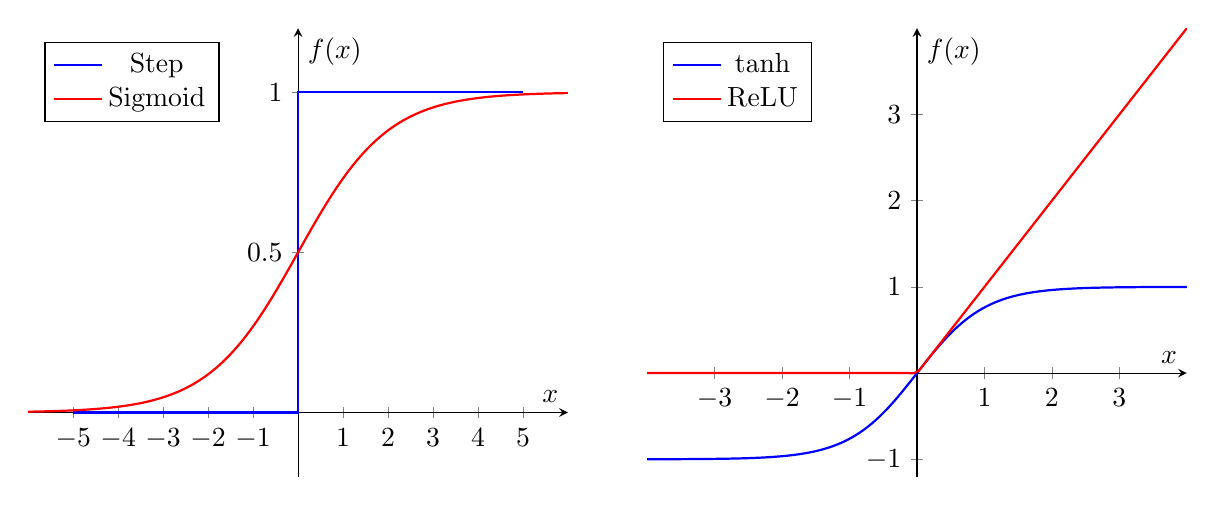
\begin{tikzpicture}

\begin{axis}[
    name=plot1,
    axis lines = middle,
    xlabel = $x$,
    ylabel = $f(x)$,
    xmin = -6, xmax = 6,
    ymin = -0.2, ymax = 1.2,
    xtick = {-5,-4,-3,-2,-1,0,1,2,3,4,5},
    ytick = {0,0.5,1},
    legend pos = north west,
    samples = 100,
    smooth,
    domain = -6:6
]
% Step function
%\addplot[blue, thick] {x < 0 ? 0 : 1};
\addplot+[const plot, no marks, thick, blue] coordinates {(-5,0) (0,0) (0,1) (5,1)};
\addlegendentry{Step}

% Sigmoid function
\addplot[red, thick] {1 / (1 + exp(-x))};
\addlegendentry{Sigmoid}

\end{axis}


\begin{axis}[
    axis lines = middle,
    at={(plot1.right of south east)},
    xshift=1cm, 
    xlabel = $x$,
    ylabel = $f(x)$,
    xmin = -4, xmax = 4,
    ymin = -1.2, ymax = 4,
    xtick = {-3,-2,-1,0,1,2,3},
    ytick = {-1,0,1,2,3},
    legend pos = north west,
    samples = 100,
    smooth,
    domain = -4:4
]

% tanh function
\addplot[blue, thick] {tanh(x)};
\addlegendentry{tanh}

% ReLU function
\addplot[red, thick] {max(0,x)};
\addlegendentry{ReLU}

\end{axis}
\end{tikzpicture}

  \captionof{figure}{Several common activation functions used with perceptrons.}
  \label{fig:activationFunctions}
 \end{tcolorbox}
\end{figure}


\subsection{Output}
The output of a perceptron is the final result of its computation, representing the neuron's decision or activation state. In the classic perceptron model, the output is typically binary, taking on values of either 0 or 1 (or sometimes -1 and 1). This binary output is determined by applying the activation function to the weighted sum of inputs. For example, if the weighted sum exceeds a certain threshold, the perceptron outputs 1; otherwise, it outputs 0. This binary nature of the output allows the perceptron to perform simple classification tasks, effectively dividing the input space into two categories. In more modern neural network architectures, the perceptron's output can be continuous, especially when using activation functions like sigmoid or hyperbolic tangent, which produce values between 0 and 1 or -1 and 1, respectively. This continuous output can be interpreted as the probability or degree of certainty of the perceptron's classification, providing more nuanced information than a strict binary decision.

\section{The Perceptron Learning Algorithm}
\subsection{Initializing The Weights}
The initialization of weights is the starting point for the model's learning process. Typically, weights are initialized to small random values, often drawn from a uniform distribution in the range $[-0.5, 0.5]$ or a normal distribution with mean 0 and small standard deviation. This randomization serves several purposes. First, it breaks symmetry, ensuring that different neurons in the network learn different features. If all weights were initialized to the same value, neurons would update identically during training, rendering them redundant. Second, small initial weights prevent the activation function from saturating at the start of training, which could slow down or halt learning. The choice of initialization method can significantly impact the perceptron's convergence speed and final performance. In some cases, more sophisticated initialization techniques, such as Xavier or He initialization, are used to maintain the variance of activations and gradients across layers, though these are more relevant for deep neural networks than for simple perceptions.

\subsection{Foreword Propagation}
Forward propagation is the process by which input signals are passed through the network, undergoing transformations at each layer until reaching the output. Forward propagation begins with the input layer, where each input value is multiplied by its corresponding weight. These weighted inputs are then summed together, often with an additional bias term. The resulting sum is passed through an activation function, which determines the perceptron's output. The output of this process represents the perceptron's decision or prediction based on the given inputs. In multi-layer networks, this process is repeated for each subsequent layer, with the outputs of one layer serving as inputs to the next, until the final output layer is reached.

\subsection{Error Calculation}
Error calculation serves as the basis for weight adjustments and overall model improvement. In the context of a perceptron, the error is typically defined as the difference between the desired output and the actual output produced by the model. For binary classification tasks, this error can be as simple as 1 (for incorrect classification) or 0 (for correct classification). In more complex scenarios, especially with continuous outputs, the error might be calculated using metrics such as mean squared error or cross-entropy. The error calculation provides a quantitative measure of the perceptron's performance, guiding the learning process. It is used to determine the direction and magnitude of weight updates during training, with larger errors generally leading to more significant adjustments. This process of error calculation and subsequent weight updating forms the core of the perceptron's ability to learn from examples and improve its classification accuracy over time.

The perceptron's learning algorithm can be categorized as a form of supervised learning, where the model is trained on labeled data pairs consisting of inputs and their corresponding desired outputs. This contrasts with unsupervised learning methods, where the model learns patterns or structures from unlabeled data without explicit target outputs. In supervised learning, the perceptron adjusts its weights based on the difference between its predicted output and the true label, aiming to minimize this error over many training examples. Unsupervised learning, on the other hand, might involve techniques like clustering or dimensionality reduction, where the goal is to discover inherent structures in the data without guidance from labeled outcomes. While the classic perceptron algorithm is supervised, variations and extensions of neural network models can incorporate both supervised and unsupervised learning principles, allowing for more flexible and powerful learning capabilities in different contexts.
\subsection{Weight Update Rule}
The weight update rule is a fundamental component of the perceptron learning algorithm, governing how the model adapts its parameters to improve performance over time. In its simplest form, the perceptron weight update rule can be expressed mathematically as:
\begin{equation}
w_i^{(t+1)}=w_i^{(t)}+\eta(y-\hat{y})x_i
\end{equation}
where $w_i^{(t)}$ is the weight for input $i$ at time step $t$, $\eta$ is the learning rate, $y$ is the true label, $\hat{y}$ is the perceptron's prediction, and $x_i$ is the input value. This rule adjusts each weight in proportion to the error $(y - \hat{y})$ and the corresponding input value $x_i$. The learning rate $\eta$ controls the size of the weight updates, balancing between quick adaptation and stability.
The intuition behind this update rule is straightforward: if the perceptron's prediction is correct ($y = \hat{y}$), no update occurs. If the prediction is incorrect, the weights are adjusted to push the output closer to the correct value. For inputs that contributed strongly to an incorrect decision (large $|x_i|$), the weight update is larger, while inputs that had little influence (small $|x_i|$) receive smaller updates. This process is repeated for each training example, gradually refining the decision boundary of the perception.

In more complex neural network architectures, this basic idea is extended to the backpropagation algorithm. Backpropagation is an algorithm used to train artificial neural networks, particularly in deep learning. It works by iteratively adjusting the weights and biases of the network to minimize the difference between the predicted output and the desired output. While the mathematical details can be complex, the core idea is simple: the network learns from its mistakes by propagating error information backwards and making small adjustments to improve its predictions over time.

\subsection{The Learning Rate}
The learning rate $\eta$ determines the size of steps taken when adjusting the weights and significantly impacts the convergence of the perceptron algorithm. A large learning rate can lead to faster convergence but risks overshooting the minimum, potentially causing the algorithm to diverge or oscillate around the optimal solution. Conversely, a small learning rate ensures more stable convergence but requires more iterations. Modern implementations often use adaptive learning rates that adjust based on the progress of learning, such as decreasing the learning rate over time or using more sophisticated optimization algorithms.

\subsection{Convergence}
Convergence in the context of perceptron learning refers to the point at which the algorithm successfully finds a set of weights that correctly classifies all training examples. In simple terms, convergence occurs when the perceptron's decision boundary accurately separates the different classes of data, and no further adjustments to the weights are needed. You know you've reached convergence when the perceptron makes no more mistakes on the training set, meaning its predictions match the true labels for all input examples. This is typically observed when the weight updates become zero or negligibly small over successive iterations. However, it's important to note that convergence is only guaranteed for linearly separable data. If the data is not linearly separable, the algorithm may never converge and could continue to oscillate between different weight configurations indefinitely.

\subsection{Linear Separability}
Linear separability refers to the ability to separate two classes of data points using a single linear decision boundary, such as a line in two dimensions or a hyperplane in higher dimensions. A dataset is considered linearly separable if there exists a linear function that can perfectly classify all data points into their respective categories. This concept is crucial for understanding the capabilities and limitations of simple neural network models, particularly the single-layer perception.

Geometrically, linear separability can be visualized as the ability to draw a straight line (in 2D) or a flat plane (in 3D) that completely separates two classes of data points (see Figure \ref{fig:linearsep}). In higher dimensions, this generalizes to a hyperplane. For instance, in a two-dimensional space, if all data points of one class can be placed on one side of a line while all points of the other class fall on the opposite side, the data is linearly separable. This geometric perspective provides an intuitive understanding of why some classification problems are solvable by simple linear models while others require more complex approaches.

\begin{figure}[h!]
\centering
\begin{tcolorbox}[every float=\centering, drop shadow, title=Linear Separability ,colback=white,colframe=WMgreen,
  colbacktitle=WMgreen,]
  \centering
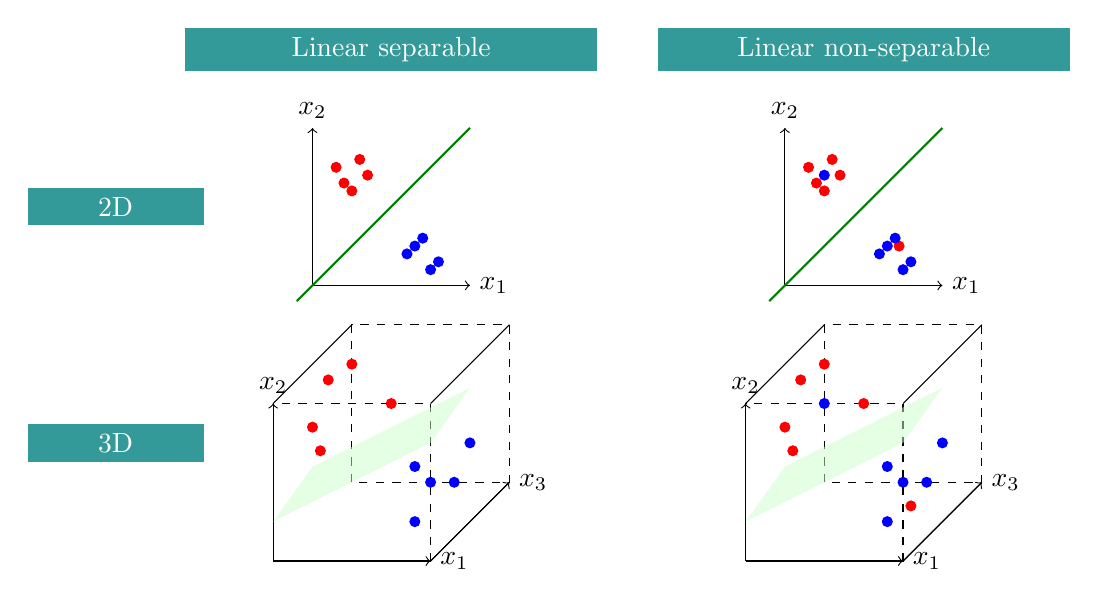
\begin{tikzpicture}
% Title row
\node[text width=5cm, align=center, fill=teal!80, text=white] 
    at (2.5,4) {Linear separable};
\node[text width=5cm, align=center, fill=teal!80, text=white] 
    at (8.5,4) {Linear non-separable};

% 2D row label
\node[text width=2cm, align=center, fill=teal!80, text=white] 
    at (-1,2) {2D};

% 2D separable plot
\begin{scope}[xshift=1.5cm, yshift=1cm]
    \draw[->] (0,0) -- (2,0) node[right] {$x_1$};
    \draw[->] (0,0) -- (0,2) node[above] {$x_2$};
    \draw[green!50!black, thick] (-0.2,-0.2) -- (2,2);
    \foreach \x/\y in {0.3/1.5, 0.5/1.2, 0.7/1.4, 0.4/1.3, 0.6/1.6}
        \fill[red] (\x,\y) circle (2pt);
    \foreach \x/\y in {1.2/0.4, 1.4/0.6, 1.6/0.3, 1.3/0.5, 1.5/0.2}
        \fill[blue] (\x,\y) circle (2pt);
\end{scope}

% 2D non-separable plot
\begin{scope}[xshift=7.5cm, yshift=1cm]
    \draw[->] (0,0) -- (2,0) node[right] {$x_1$};
    \draw[->] (0,0) -- (0,2) node[above] {$x_2$};
    \draw[green!50!black, thick] (-0.2,-0.2) -- (2,2);
    \foreach \x/\y in {0.3/1.5, 0.5/1.2, 0.7/1.4, 0.4/1.3, 0.6/1.6, 1.45/.5}
        \fill[red] (\x,\y) circle (2pt);
    \foreach \x/\y in {1.2/0.4, 1.4/0.6, 1.6/0.3, 1.3/0.5, 1.5/0.2, 0.5/1.4}
        \fill[blue] (\x,\y) circle (2pt);
    %\fill[red] (1.4/0.5) circle (2pt);
    %\draw[->, black] (0.5,1.5) -- (0.5,1.3);
    %\draw[->, black] (1.4,0.6) -- (1.4,0.4);
\end{scope}

% 3D row label
\node[text width=2cm, align=center, fill=teal!80, text=white] 
    at (-1,-1) {3D};

% 3D separable plot
\begin{scope}[xshift=1cm, yshift=-2.5cm]
    \draw[dashed] (0,0) -- (0,2) -- (2,2) -- (2,0) -- cycle;
    \draw[->, black] (0,0) -- (2,0) node[right] {$x_1$};
    \draw[->, black] (0,0) -- (0,2) node[above] {$x_2$};
    \draw[->, black] (2,0) -- (3,1) node[right] {$x_3$};
    \draw (2,0) -- (3,1);
    \draw (0,2) -- (1,3);
    \draw (2,2) -- (3,3);
    \draw[dashed] (1,1) -- (1,3) -- (3,3) -- (3,1) -- cycle;
    \fill[green!20, opacity=0.5] (0,0.5) -- (2,1.5) -- (2.5,2.2) -- (0.5,1.2) -- cycle;
    \foreach \x/\y in {0.5/1.7, 1/2.5, 1.5/2, .7/2.3, .6/1.4}
        \fill[red] (\x,\y) circle (2pt);
    \foreach \x/\y in {2/1, 2.5/1.5, 1.8/1.2, 1.8/.5, 2.3/1}
        \fill[blue] (\x,\y) circle (2pt);
\end{scope}

% 3D non-separable plot
\begin{scope}[xshift=7cm, yshift=-2.5cm]
    \draw[dashed] (0,0) -- (0,2) -- (2,2) -- (2,0) -- cycle;
    \draw[->, black] (0,0) -- (2,0) node[right] {$x_1$};
    \draw[->, black] (0,0) -- (0,2) node[above] {$x_2$};
    \draw[->, black] (2,0) -- (3,1) node[right] {$x_3$};
    \draw (2,2) -- (3,3);
    \draw (2,0) -- (3,1);
    \draw (0,2) -- (1,3);
    \draw[dashed] (1,1) -- (1,3) -- (3,3) -- (3,1) -- cycle;
    \fill[green!20, opacity=0.5] (0,0.5) -- (2,1.5) -- (2.5,2.2) -- (0.5,1.2) -- cycle;
    \foreach \x/\y in {0.5/1.7, 1/2.5, 1.5/2, .7/2.3, .6/1.4, 2.1/.7}
        \fill[red] (\x,\y) circle (2pt);
    \foreach \x/\y in {2/1, 2.5/1.5, 1.8/1.2, 1.8/.5, 2.3/1, 1/2}
        \fill[blue] (\x,\y) circle (2pt);
\end{scope}

\end{tikzpicture}
  \captionof{figure}{Examples of linear separable and linear non-separable classes of data in both two and three dimensions.}
  \label{fig:linearsep}
 \end{tcolorbox}
\end{figure}

\subsection{The Bias Parameter}
In our earlier discussions of the perceptron, we simplified the model by focusing on the weights and inputs alone. However, there is an additional ``bias'' term that is an important component of the perceptron's architecture. Without a bias term, the decision boundary would always be constrained to pass through the origin (0,0), severely limiting the perceptron's classification capabilities. Think of the bias as shifting the decision boundary - much like how the green line in the 2D visualizations in Figure \ref{fig:linearsep} can be moved up or down to better separate the red and blue points.

Mathematically, the bias (b) acts as an additional term in the weighted sum: $\sum_{i=1}^n(w_ix_i)+b$, where it effectively determines the perceptron's threshold for activation. The bias can be thought of as adjusting the "default" response of the perceptron - it determines how easily the neuron "fires" regardless of the input values. During training, the bias is updated along with the weights using the same learning rule: $b_{new}=b_{old}-\eta(y-\hat{y})$, where $\eta$ is the learning rate, $y$ is the true label, and $\hat{y}$ is the predicted output. This allows the perceptron to find the optimal position for its decision boundary in the input space.
 
\subsection{Multi-layer Perceptrons}
Multi-layer perceptrons (MLPs), consisting of multiple layers of "neurons" emerged as a solution to overcome the limitations of single-layer perceptrons, particularly in solving non-linearly separable problems. MLPs contain one or more hidden layers between the input and output layers (see Figure \ref{multilayer}). This architecture enables MLPs to solve non-linearly separable problems that were impossible for single-layer perceptrons to handle. Each layer in an MLP consists of multiple artificial neurons, with each neuron connected to every neuron in the subsequent layer, forming a fully connected feedforward network. 
\begin{figure}[H]
\centering
\begin{tcolorbox}[every float=\centering, drop shadow, title=Multi-layer Perceptrons ,colback=white,colframe=WMgreen,
  colbacktitle=WMgreen,]
  \centering
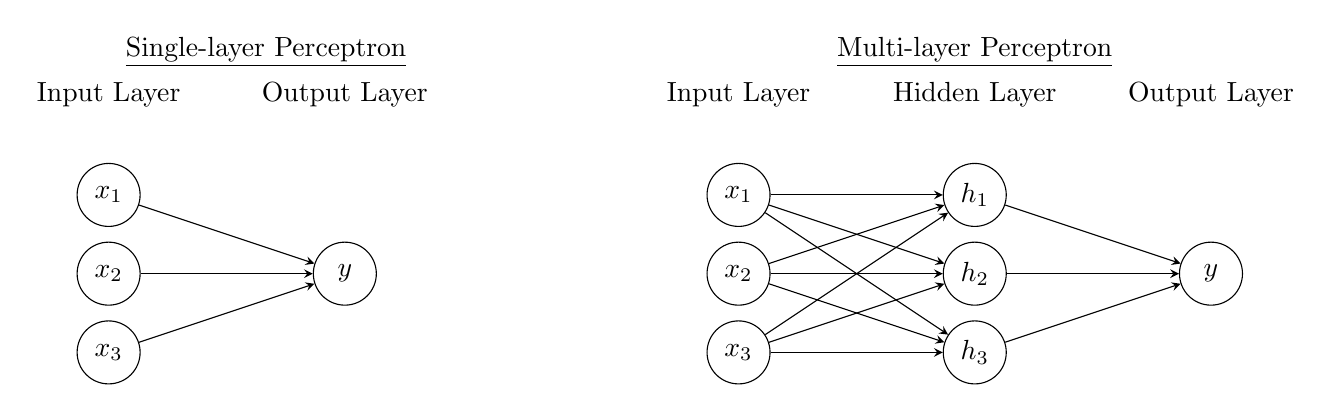
\begin{tikzpicture}[
    neuron/.style={circle, draw, minimum size=0.8cm},
    >=stealth,
    node distance=2cm
]
% Two-layer perceptron
\begin{scope}
    % Input layer
    \foreach \i in {1,2,3} {
        \node[neuron] (i\i) at (0,-\i) {$x_\i$};
    }
    
    % Output layer
    \node[neuron] (o1) at (3,-2) {$y$};
    
    % Connections
    \foreach \i in {1,2,3} {
        \draw[->] (i\i) -- (o1);
    }
    
    % Labels
    \node[above] at (0,0) {Input Layer};
    \node[above] at (3,0) {Output Layer};
    \node[above] at (2,.5) {\underline{Single-layer Perceptron}};
\end{scope}

% Three-layer perceptron
\begin{scope}[xshift=8cm]
    % Input layer
    \foreach \i in {1,2,3} {
        \node[neuron] (i\i) at (0,-\i) {$x_\i$};
    }
    
    % Hidden layer
    \foreach \i in {1,2,3} {
        \node[neuron] (h\i) at (3,-\i) {$h_\i$};
    }
    
    % Output layer
    \node[neuron] (o1) at (6,-2) {$y$};
    
    % Connections
    \foreach \i in {1,2,3} {
        \foreach \j in {1,2,3} {
            \draw[->] (i\i) -- (h\j);
        }
    }
    \foreach \i in {1,2,3} {
        \draw[->] (h\i) -- (o1);
    }
    
    % Labels
    \node[above] at (0,0) {Input Layer};
    \node[above] at (3,0) {Hidden Layer};
    \node[above] at (6,0) {Output Layer};
    \node[above] at (3,.5) {\underline{Multi-layer Perceptron}};
\end{scope}

\end{tikzpicture}
  \caption{Examples of both a simple, single-layer perception and a multi-layer perception with one hidden layer.}
  \label{fig:multilayer}
 \end{tcolorbox}
\end{figure}

The power of MLPs lies in their ability to learn complex, non-linear mappings between inputs and outputs through the process of backpropagation. The hidden layers transform the input space into increasingly abstract representations, allowing the network to capture intricate patterns in the data. For example, in a classification task, the first hidden layer might learn simple features, while subsequent layers combine these features into more complex representations. This hierarchical feature learning enables MLPs to approximate any continuous function with arbitrary precision, a property known as universal function approximation. The number of hidden layers and neurons in each layer can be adjusted to balance between the network's capacity to learn complex patterns and its ability to generalize to new data. While single-layer perceptrons are now primarily used for teaching neural network concepts and solving simple linear classification problems, their theoretical foundations continue to influence the design and understanding of more complex neural architectures used in contemporary pattern recognition, computer vision, and machine learning applications.

\section{Build Your Own Perceptron}
Now that you have a general understanding about perceptions and their underlying computational principles, you can build our own perception using a simple spreadsheet application like MS Excel, or Google Sheets. In this example, we will build a perceptron that learns to recognize if a face is happy or sad based on two features:
\begin{enumerate}
\item Mouth curve ($x_1$): Positive (+1) for a smile, negative (-1) for a frown.
\item Eye openness ($x_2$): Positive (+1) for wide-open eyes, and negative (-1) for narrow eyes.
\end{enumerate}
\vspace{.2cm}
\noindent The perception (depicted in Figure \ref{fig:firstperceptron}) will classify faces as \textbf{Happy} ($y=1$) or \textbf{Sad}($y=0$). 

\begin{figure}[h!]
\centering
\begin{tcolorbox}[every float=\centering, drop shadow, title=Your First Perceptron ,colback=white,colframe=WMgreen,
  colbacktitle=WMgreen,]
  \centering
\begin{tikzpicture}
  % Input nodes (simplified face representations)
  \node[circle,draw,align=center] (input1) at (0,2) {$x_1$ \\ {\tiny{Mouth}}};
  \node[circle,draw,align=center] (input2) at (0,0) {$x_2$ \\ {\tiny{Eyes}}};
  \node[circle,draw,align=center] (bias)   at (1,-1.5) {$b$};
  
  % Output node
  \node[circle,draw] (output) at (4,1) {$\sum_{i=1}^2w_ix_i+b$};
  % Activation function
  \node[draw, rectangle, minimum size=1.2cm, right=1cm of output] (act) {Step};
  % Output
  \node[draw, circle, minimum size=1cm, right=1cm of act] (yhat) {$\hat{y}$};
  
  % Connections
  \draw[->] (input1) -- node[above] {$w_1$} (output);
  \draw[->] (input2) -- node[below] {$w_2$} (output);
  \draw[->] (output) -- (act);
  \draw[->] (act) -- (yhat);
  \draw[->] (bias) -- (output);
  
  % Labels
  \node[left] at (-1,1) {Inputs};
  \node[right=.5cm of yhat] {Output};
\end{tikzpicture}
  \captionof{figure}{Illustration of a simple perception that can learn to distinguish happy and sad faces based on two features: (1) the curvature of the mouth and (2) the openness of the eyes. Also depicted are the bias parameter and the step activation function that will be used.}
  \label{fig:firstperceptron}
 \end{tcolorbox}
\end{figure}

\subsection{Set Up The Spreadsheet}
Set up the components needed to build and train your perception (see Table \ref{tab:perceptron_setup}).  You will need to designate columns for the two inputs $x_1$(Mouth Curve) and $x_2$(Eye Openness), and add some training stimuli with different values for the two inputs (e.g., facial features).  Next, designate a column for the True Label and then enter the correct label for each of your inputs (happy=1, sad=0). You will also need weights for each of your inputs (e.g., $w_1$ \& $w_2$) and a column for the bias ($b$) and learning rate ($\eta$) parameters.  Finally, you will need columns for the perceptron's output, including the weighted sum (i.e., $\sum_{i=1}^nw_ix_i+b$), the output (the perceptron's prediction), and the calculated error (i.e., $(y-\hat y$).  An example of the column layout is presented in Table \ref{tab:perceptron_setup} with initial values entered for the weights, bias, and learning rate parameters (note that the learning rate remains constant in this example).
\begin{table}[h!]
\centering
\fontsize{9}{12}\selectfont % Reduces the font size of the table
\begin{tabular}{@{}|c|c|c|c|c|c|c|c|c|c|@{}}
\hline
\rowcolor{gray!30}\textbf{A} & \textbf{B} & \textbf{C} & \textbf{D} & \textbf{E} & \textbf{F} & \textbf{G} & \textbf{H} & \textbf{I} & \textbf{J} \\ \hline
\textbf{$x_1$(Mouth Curve)} & \textbf{$x_2$(Eye Openness)} & \textbf{True Label} & \textbf{$w_1$} & \textbf{$w_2$} & \textbf{$b$} & \textbf{$\eta$} & \textbf{Weighted Sum} & \textbf{Prediction} & \textbf{Error} \\ \hline
1.0                          & 1.0                           & 1                      & 0.5                 & 0.5                & 0.2     &0.01        & -                      & -                     & -                 \\ \hline
-1.0                         & 1.0                           & 0                      & -                 & -                & -     &0.01        & -                      & -                     & -                 \\ \hline
1.0                          & -1.0                           & 1                      & -                 & -                & -     &0.01        & -                      & -                     & -                 \\ \hline
-1.0                         & -1.0                           & 0                      & -                 & -                & -     &0.01        & -                      & -                     & -                 \\ \hline
\end{tabular}
\caption{Column Layout for the Perceptron}
\label{tab:perceptron_setup}
\end{table}

Next, use a formula to calculate the weighted sum $\sum_{i=1}^nw_ix_i+b$.  If your columns are set up like Table \ref{tab:perceptron_setup} then the formula below will work in either Excel or Google Sheets. You can copy this formula into all rows.
\[
=A2 * D2 + B2 * E2 + F2
\]

Now, Use the step function to determine if the perceptron thinks the face is happy (1) or sad (0). This can be implemented using the $if()$ function in either Excel or Google Sheets.  If your weighted sums are in column G as they are in Table \ref{tab:perceptron_setup}, then the step function would be implemented using the following formula in cell I2:
\[
= IF(G2 >= 0, 1, 0)
\]

Finally, calculate the error ($y-\hat y$).  This will simply be the difference between the value in the True Label column and the Prediction column. In the present example, that means that the formula in cell J2 will be:
\[
= C2 - H2
\]

\subsection{Training The Perceptron}
Once the architecture of your perception is established, it is time to start updating the weights based on the errors in prediction on the initial training case (i.e., row 1).  To do this, we will apply the perception learning rule to the initial values in the $w1$, $w2$, and bias ($b$) columns.  Recall that the perceptron learning rule to update the weights is $w_i^{(updated)}=w_i^{(old)}+\eta(y-\hat{y})x_i$. Continuing with the example in table \ref{tab:perceptron_setup}, use the formulae:
\begin{alignat*}{3}
&\text{Cell D3} &&= w_1^{(updated)} &&= D2+G2*J2*A2 \text{\hspace{.3cm}} \\
&\text{Cell E3} &&= w_2^{(updated)} &&= E2+G2*J2*B2 \text{\hspace{.3cm}} \\
&\text{Cell F3} &&= b^{(updated)} &&= F2+G2*J2  \text{\hspace{.3cm}}
\end{alignat*}

Now that you have calculated the updated weights and bias after the perceptron has had a chance to "learn" from the initial sampled values for Mouth Curve and Eye Openness in row 2, copy the formula above across the remaining rows, being sure to use dynamic references so that the updated values of .  Be careful NOT to copy/paste the updated cells because that will copy the formula rather than the updated values of $w1$, $w2$, and bias ($b$) in row 4 are based on the values in row 3 etc. If you have entered the formula exactly as they are shown in this example, you can simply copy the formula for $w1$, $w2$, and bias ($b$) to each subsequent row. 

In this illustrated example, the perception has really only had three chances to ``learn'' how to distinguish happy and sad faces.  In practice, it will take more than just a few instances or ``trials'' before the perception has converged on a stable solution.  Convergence in perceptron training refers to the process by which the weights and bias reach stable values that correctly classify all training examples. For linearly separable data, the perceptron convergence theorem guarantees that the learning algorithm will eventually find a solution in a finite number of steps, regardless of the initial weights. However, for data that is not linearly separable, the perceptron will never converge as the weights will continue to update without finding a perfect solution. The convergence process involves iteratively adjusting weights and bias in response to classification errors, with each update moving the decision boundary closer to an optimal position. The rate of convergence is influenced by several factors including the learning rate, the initial weight values, and the geometric arrangement of the training data points. When the data points are well-separated, convergence typically occurs more quickly than when the points are close to the decision boundary. 

The sequence of training during which the perception from one instance of each set of inputs in the training set is sometimes called an epoch.  In the present case, one epoch consists of training the perception on each of the four ``faces'' in the training set. Given the data points and initial weights, bias, and learning rate illustrated in table \ref{tab:perceptron_setup}, this perception should converge after about seven epochs, when it will be able to perfectly classify each of the four faces in the training set. 

\subsection{Understanding the Decision Boundary}
A decision boundary in a perceptron represents the line (in 2D) or hyperplane (in 3D or higher dimensions) that separates different classes of data points based on the learned weights and bias. For a two-input perceptron, this boundary is defined by the equation $w_1x_1 + w_2x_2 + b = 0$, where $w_1$ and $w_2$ are the weights, $x_1$ and $x_2$ are the inputs, and $b$ is the bias term. When a point falls on one side of this boundary (weighted sum $\geq$ 0), the perceptron outputs 1, and when it falls on the other side (weighted sum $<$ 0), it outputs 0. During training, the perceptron adjusts its weights and bias to position this decision boundary optimally between the classes. Remember, the perceptron can only successfully separate classes when they are linearly separable, meaning a single straight line (or hyperplane) can be drawn to separate all positive examples (e.g., happy faces) from all negative examples (e.g., sad faces).  The initial decision boundary for the two-input perception developed in the previous section is illustrated in figure \ref{fig:initdecisionbound}.  Notice that with the initial values of $w_1=0.5$, $w_2=0.5$, and $b=0.2$, the perception will incorrectly output 1 when $x_1$ (Mouth Curve) = -1 and $x_2$ (Eye Openness) = 1.

\begin{figure}[h!]
\centering
\begin{tcolorbox}[every float=\centering, drop shadow, title=Initial Decision Boundary (Before Training),colback=white,colframe=WMgreen,
  colbacktitle=WMgreen,]
  \centering
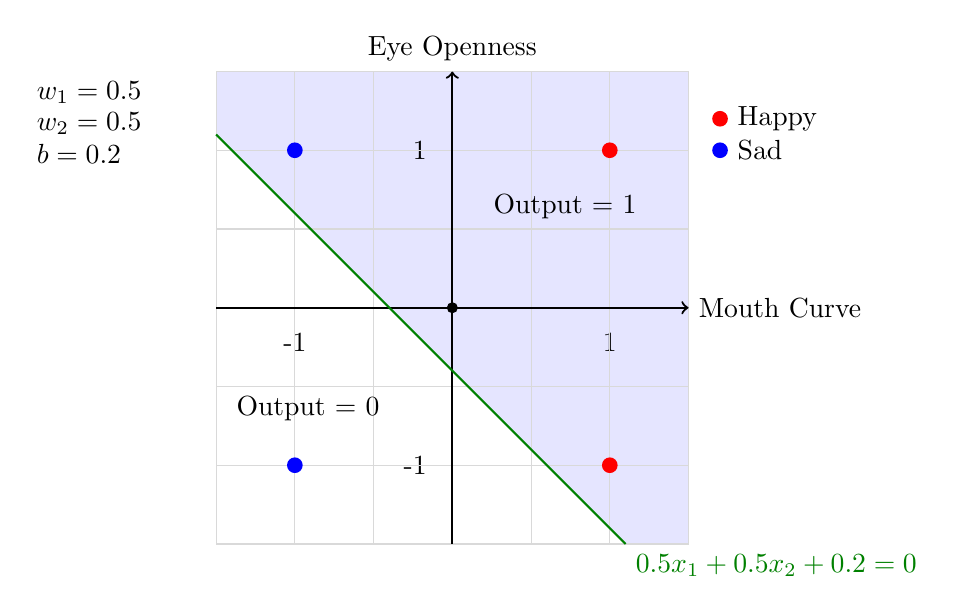
\begin{tikzpicture}[scale=2]

    \begin{scope}
    \clip (-1.5,-1.5) rectangle (1.5,1.5);
        \fill[blue!10] (-1.5,1.1) -- (1.5,-1.9) -- (1.5,1.5) -- (-1.5,1.5) -- cycle;
    \end{scope}
    
    % Tick marks and labels
    \draw (-1,0.1) -- (-1,-0.1) node[below] {-1};
    \draw (1,0.1) -- (1,-0.1) node[below] {1};
    \draw (0.1,-1) -- (-0.1,-1) node[left] {-1};
    \draw (0.1,1) -- (-0.1,1) node[left] {1};
    
    % Grid
    \draw[gray!30, step=0.5] (-1.5,-1.5) grid (1.5,1.5);

    % Axes with labels
    \draw[->,thick] (-1.5,0) -- (1.5,0) node[right] {Mouth Curve};
    \draw[->,thick] (0,-1.5) -- (0,1.5) node[above] {Eye Openness};
    
    % Point at origin
    \fill[black] (0,0) circle (1pt);

    % Decision boundary line: 0.5x₁ + 0.5x₂ + 0.2 = 0
    % Solving for x₂: x₂ = -x₁ - 0.4   
    \draw[thick, green!50!black] (-1.5,1.1) -- (1.1,-1.5) 
        node[below right] {$0.5x_1 + 0.5x_2 + 0.2 = 0$};
    
    % Label regions
    \node[above right] at (0.2,0.5) {Output = 1};
    \node[below left] at (-0.4,-0.5) {Output = 0};

    % Training data points
    \node[circle, fill=red, inner sep=2pt] at (1,1) {};
    \node[circle, fill=blue, inner sep=2pt] at (-1,1) {};
    \node[circle, fill=red, inner sep=2pt] at (1,-1) {};
    \node[circle, fill=blue, inner sep=2pt] at (-1,-1) {};

    % Legend
    \node[circle, fill=red, inner sep=2pt] at (1.7,1.2) {};
    \node[right] at (1.75,1.2) {Happy};
    \node[circle, fill=blue, inner sep=2pt] at (1.7,1.0) {};
    \node[right] at (1.75,1.0) {Sad};
    
    % Add parameters
    \node[below right] at (-2.7,1.5) {$w_1 = 0.5$};
    \node[below right] at (-2.7,1.3) {$w_2 = 0.5$};
    \node[below right] at (-2.7,1.1) {$b = 0.2$};
\end{tikzpicture}
  \captionof{figure}{Illustration of the initial decision boundary for the two-input perception with initial values of $w_1=0.5$, $w_2=0.5$, and $b=0.2$.}
  \label{fig:initdecisionbound}
 \end{tcolorbox}
\end{figure}

However, once the perception has had the opportunity to learn from a training set and make adjustments to the values of $w_1$, $w_2$, and $b$ using the perception learning rule, it will adjust the decision boundary so that only the two exemplars in the training set that were labeled ``Happy'' will result in an output of 1, indicating that the perception's classification of an input as happy.  For example, training the two-input perceptron from above might result in $w_1=0.57$, $w_2=0.43$, and $b=0.13$, which would result in the decision boundary pictured in figure \ref{fig:traindecisionbound}.

\begin{figure}[h!]
\centering
\begin{tcolorbox}[every float=\centering, drop shadow, title=Decision Boundary After Training,colback=white,colframe=WMgreen,
  colbacktitle=WMgreen,]
  \centering
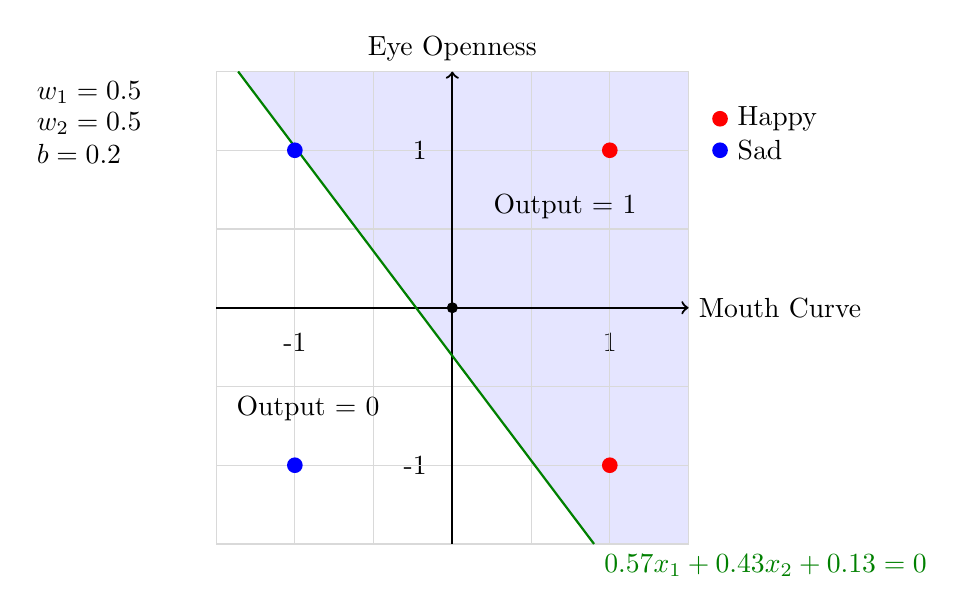
\begin{tikzpicture}[scale=2]

    \begin{scope}
    \clip (-1.5,-1.5) rectangle (1.5,1.5);
        \fill[blue!10] (-1.5,1.687) -- (1.5,-2.291) -- (1.5,1.5) -- (-1.5,1.5) -- cycle;
    \end{scope}
    
    % Tick marks and labels
    \draw (-1,0.1) -- (-1,-0.1) node[below] {-1};
    \draw (1,0.1) -- (1,-0.1) node[below] {1};
    \draw (0.1,-1) -- (-0.1,-1) node[left] {-1};
    \draw (0.1,1) -- (-0.1,1) node[left] {1};
    
    % Grid
    \draw[gray!30, step=0.5] (-1.5,-1.5) grid (1.5,1.5);

    % Axes with labels
    \draw[->,thick] (-1.5,0) -- (1.5,0) node[right] {Mouth Curve};
    \draw[->,thick] (0,-1.5) -- (0,1.5) node[above] {Eye Openness};
    
    % Point at origin
    \fill[black] (0,0) circle (1pt);

    % Decision boundary line: 0.5x₁ + 0.5x₂ + 0.2 = 0
    % Solving for x₂: x₂ = -x₁ - 0.4   
    \draw[thick, green!50!black] (-1.36,1.5) -- (0.90,-1.5) 
        node[below right] {$0.57x_1 + 0.43x_2 + 0.13 = 0$};
    
    % Label regions
    \node[above right] at (0.2,0.5) {Output = 1};
    \node[below left] at (-0.4,-0.5) {Output = 0};

    % Training data points
    \node[circle, fill=red, inner sep=2pt] at (1,1) {};
    \node[circle, fill=blue, inner sep=2pt] at (-1,1) {};
    \node[circle, fill=red, inner sep=2pt] at (1,-1) {};
    \node[circle, fill=blue, inner sep=2pt] at (-1,-1) {};

    % Legend
    \node[circle, fill=red, inner sep=2pt] at (1.7,1.2) {};
    \node[right] at (1.75,1.2) {Happy};
    \node[circle, fill=blue, inner sep=2pt] at (1.7,1.0) {};
    \node[right] at (1.75,1.0) {Sad};
    
    % Add parameters
    \node[below right] at (-2.7,1.5) {$w_1 = 0.5$};
    \node[below right] at (-2.7,1.3) {$w_2 = 0.5$};
    \node[below right] at (-2.7,1.1) {$b = 0.2$};
\end{tikzpicture}
  \captionof{figure}{Illustration of the decision boundary for the two-input perception after training $w_1=0.57$, $w_2=0.43$, and $b=0.13$.}
  \label{fig:traindecisionbound}
 \end{tcolorbox}
\end{figure}

\begin{table}[h!]
\centering
%\fontsize{12}{12}\selectfont % Reduces the font size of the table
\begin{tabular}{@{}|c|c|c|@{}}
\hline
\rowcolor{gray!30}\textbf{A} & \textbf{B} & \textbf{C}  \\ \hline
\textbf{$x_1$(Mouth Curve)} & \textbf{$x_2$(Eye Openness)} & \textbf{True Label} \\ \hline
1 & 1.5 & 1(Happy) \\ \hline
-1.2 & .8 & 0(Sad) \\ \hline
\end{tabular}
\caption{Test data for the trained perceptron}
\label{tab:perceptron_test}
\end{table}

Notice that the perceptron learning algorithm stops as soon as all training examples are correctly classified, even if some points lie very close to the decision boundary. This early stopping behavior means that while the final weights ($w_1 = 0.57$, $w_2 = 0.43$, $b = 0.13$) achieve perfect classification of the training data, the solution may not be optimal in terms of margin or robustness. For example, a point that is correctly classified but sits very near the decision boundary could easily be misclassified if there's any noise in the input features. The algorithm is satisfied with any solution that achieves linear separation, rather than searching for the solution that maximizes the distance between the decision boundary and the closest training points. This is one of the key limitations of the perceptron learning rule - it guarantees convergence for linearly separable data, but doesn't guarantee finding the most stable or generalizable solution.

\section{A Pyschological Interpretation of the Perceptron}
\subsection{Attention}
The weights learned by a perceptron can be interpreted as a simple form of attention or feature importance in the classification task. When a perceptron converges to a solution, the magnitude of each weight reflects how much the model "pays attention to" or relies on its corresponding input feature to make decisions.
For example, in a face classification task where $x_1$ represents mouth curvature and $x_2$ represents eye openness, if $w_1 = 0.57$ and $w_2 = 0.43$, the perceptron has learned to pay more attention to the mouth feature than the eye feature when determining if a face is happy or sad. The larger magnitude of $w_1$ indicates that mouth curvature is more predictive of the emotional expression, while the smaller $w_2$ suggests that eye openness contributes less to the classification decision.

This attention mechanism, though primitive compared to modern neural networks, demonstrates how machine learning models can automatically discover which features are most relevant for a given task. When a weight approaches zero, it effectively means the perceptron has learned to ignore that input feature, while larger weights (positive or negative) indicate features that strongly influence the output. The bias term then acts as a threshold adjuster, determining how the weighted combination of these attended features translates into the final classification decision.

\subsection{Learning}
The perceptron's learning mechanism mirrors several fundamental principles of human learning and cognitive psychology. The weight update rule, where connections are strengthened or weakened based on experience, closely parallels Hebbian learning theory's principle that "neurons that fire together, wire together." Just as humans strengthen neural pathways through repeated exposure and practice, the perceptron adjusts its weights through iterative training experiences, strengthening connections that lead to correct predictions and weakening those that lead to errors.

The error-driven nature of perceptron learning also reflects psychological theories of learning through feedback and correction. When humans make mistakes, they adjust their behavior based on the error signal, much like how the perceptron updates its weights proportionally to the error term. This process of gradual refinement through trial and error mirrors how humans learn complex tasks, starting with imperfect performance and gradually improving through experience and feedback. The perceptron's bias term serves a similar function to cognitive biases in human decision-making, creating a baseline tendency or threshold that must be overcome before making a particular choice.

The perceptron's ability to learn from examples rather than explicit rules also reflects how humans often learn through pattern recognition and generalization rather than formal instruction. Just as humans can learn to categorize objects or situations based on repeated exposure to examples, the perceptron develops its classification ability by extracting patterns from training data. This parallel between artificial and biological learning mechanisms helps explain why early perceptron research was so influential in both computer science and cognitive psychology, establishing fundamental principles that continue to influence our understanding of both artificial and natural learning systems.

\subsection{Modern Applications}
Modern applications of perceptrons extend far beyond their original role in binary classification, serving as fundamental building blocks in more sophisticated neural architectures and practical applications. In computer vision and image processing, perceptron-based feature detectors help identify edges, patterns, and basic shapes that form the foundation for more complex object recognition tasks. These simple neural units are also used in automated quality control systems, where they can rapidly classify products as acceptable or defective based on visual or sensor inputs.

The perceptron's interpretable nature - with weights directly indicating feature importance - makes it valuable in fields like medical diagnostics and financial risk assessment, where understanding the decision-making process is crucial. For example, perceptrons can help identify which symptoms or financial indicators most strongly predict particular outcomes. In robotics and control systems, arrays of perceptrons work together to process sensor data and make real-time decisions about movement and navigation. The perceptron's efficiency and speed in binary classification also makes it useful in preliminary data filtering for more complex AI systems, helping to reduce computational load by quickly identifying and filtering out clearly irrelevant inputs before more sophisticated processing takes place.

\newpage
\section{Three-Input Perceptron Design Project}

\noindent\textbf{Overview}\\
In this assignment, you will extend your understanding of perceptron learning by implementing a three-input perceptron. \textbf{Choose ONE of the scenarios below.} Each scenario represents a real-world decision process that can be modeled as a binary classification problem, making them ideal for perceptron learning while being relatable to students' daily experiences. Like biological neurons that become tuned to specific input patterns, the perceptron learns to "pay attention" to relevant features by adjusting their weights. For example, in the library decision scenario, if having an exam tomorrow ($x_1$) consistently leads to studying, the weight $w_1$ becomes larger, similar to how sensory neurons become more responsive to important stimuli. The perceptron's binary activation threshold is similar to the way neurons only fire when their inputs exceed a certain threshold. This simple learning model helps explain how networks of biological neurons might learn to make decisions through gradual adjustment of their connections based on experience and feedback.

\vspace{0.4cm}
\noindent\textbf{Option 1: Library Decision}\\
You are trying to understand the factors that contribute to a student's decision to go to the library. Your perceptron will learn to predict whether a student will choose to study at the library based on three key factors: whether they have an exam the next day, if their friends are studying there, and their current energy level. The perceptron should learn which factors are most influential in this decision-making process.\\
Inputs:
\begin{itemize}
\item $x_1$: Exam tomorrow (1 = yes, -1 = no)
\item $x_2$: Friends studying there (1 = yes, -1 = no)
\item $x_3$: Have energy/caffeine (1 = yes, -1 = no)
\end{itemize}
Output: Go to library (1) or stay home (0)

\vspace{0.4cm}
\noindent\textbf{Option 2: Party Decision}\\
You want to model how students decide whether to attend a weekend party. Your perceptron will weigh three competing factors: whether there's homework due the next day (responsibility), if close friends are attending (social pressure), and whether they have enough money for the event (practical constraint). Through training, the perceptron will reveal which factors most strongly influence the go/no-go decision.\\
Inputs:
\begin{itemize}
\item $x_1$: Homework due tomorrow (1 = yes, -1 = no)
\item $x_2$: Close friends attending (1 = yes, -1 = no)
\item $x_3$: Have money for event (1 = yes, -1 = no)
\end{itemize}
Output: Go to party (1) or stay home (0)

\vspace{0.4cm}
\noindent\textbf{Option 3: Morning Workout}\\
You're investigating what determines whether someone will follow through with their morning exercise plan. Your perceptron will analyze three common factors: quality of sleep the night before, weather conditions, and whether their workout partner is committed to showing up. The trained weights will show which factors are most crucial in maintaining exercise consistency.\\
Inputs:
\begin{itemize}
\item $x_1$: Got enough sleep (1 = yes, -1 = no)
\item $x_2$: Weather is good (1 = yes, -1 = no)
\item $x_3$: Workout buddy committed (1 = yes, -1 = no)
\end{itemize}
Output: Go exercise (1) or skip today (0)

\newpage
\begin{center} \large Report Form \end{center}\par
\noindent\textbf{Name}\\
\noindent \framebox[.9\textwidth][l]{\rule{0pt}{1cm}}

\noindent\textbf{Which option did you choose?}\\
\noindent \framebox[.9\textwidth][l]{\rule{0pt}{1cm}}

\vspace{0.4cm}
\begin{minipage}{0.4\textwidth}
\noindent\textbf{Initial Parameters:}\\
\begin{tabular}{|l|c|}
\hline
Initial weight $w_1$ & \framebox[2cm][l]{\rule{0pt}{.5cm}} \\
Initial weight $w_2$ & \framebox[2cm][l]{\rule{0pt}{.5cm}} \\
Initial weight $w_3$ & \framebox[2cm][l]{\rule{0pt}{.5cm}} \\
Initial bias $b$ & \framebox[2cm][l]{\rule{0pt}{.5cm}} \\
Learning rate $\eta$ & \framebox[2cm][l]{\rule{0pt}{.5cm}} \\
\hline
\end{tabular}
\end{minipage}
%\hfill
\begin{minipage}{0.4\textwidth}
\textbf{Training Data:}\\
\begin{tabular}{|c|c|c|c|}
\hline
$x_1$ & $x_2$ & $x_3$ & Target \\
\hline
\framebox[2cm][l]{\rule{0pt}{.5cm}} & \framebox[2cm][l]{\rule{0pt}{.5cm}} & \framebox[2cm][l]{\rule{0pt}{.5cm}} & \framebox[2cm][l]{\rule{0pt}{.5cm}} \\
\framebox[2cm][l]{\rule{0pt}{.5cm}} & \framebox[2cm][l]{\rule{0pt}{.5cm}} & \framebox[2cm][l]{\rule{0pt}{.5cm}} & \framebox[2cm][l]{\rule{0pt}{.5cm}} \\
\framebox[2cm][l]{\rule{0pt}{.5cm}} & \framebox[2cm][l]{\rule{0pt}{.5cm}} & \framebox[2cm][l]{\rule{0pt}{.5cm}} & \framebox[2cm][l]{\rule{0pt}{.5cm}} \\
\framebox[2cm][l]{\rule{0pt}{.5cm}} & \framebox[2cm][l]{\rule{0pt}{.5cm}} & \framebox[2cm][l]{\rule{0pt}{.5cm}} & \framebox[2cm][l]{\rule{0pt}{.5cm}} \\
\framebox[2cm][l]{\rule{0pt}{.5cm}} & \framebox[2cm][l]{\rule{0pt}{.5cm}} & \framebox[2cm][l]{\rule{0pt}{.5cm}} & \framebox[2cm][l]{\rule{0pt}{.5cm}} \\
\framebox[2cm][l]{\rule{0pt}{.5cm}} & \framebox[2cm][l]{\rule{0pt}{.5cm}} & \framebox[2cm][l]{\rule{0pt}{.5cm}} & \framebox[2cm][l]{\rule{0pt}{.5cm}} \\
\hline
\end{tabular}
\end{minipage}

\vspace{0.5cm}
\noindent\textbf{Linear Separability Analysis}\\
Use the 3D graphing calculator at \url{https://www.desmos.com/3d} to plot your training data.  Take a screenshot of your plot and paste it below. Give a brief explanation as to why your chosen points are linearly separable.  You can also use the formula describing your initial decision boundary to plot the corresponding hyperplane.\\
\framebox[\textwidth][l]{\rule{0pt}{9cm}}
\textit{NOTE: enter data points using the syntax, ``(1, 1, 1)'' and enter formula using the syntax, ``$y=.5x+.5y+.5z+.2$'', where $x$, $y$, \& $z$ correspond with the perceptron's inputs, $x_1$, $x_2$, \& $x_3$.}
\newpage

\vspace{0.5cm}
\noindent\textbf{Final Results}
\begin{center}
\begin{tabular}{|r|c|}
\hline
Final $w_1$ & \framebox[2cm][l]{\rule{0pt}{.5cm}} \\
Final $w_2$ & \framebox[2cm][l]{\rule{0pt}{.5cm}} \\
Final $w_3$ & \framebox[2cm][l]{\rule{0pt}{.5cm}} \\
Final bias & \framebox[2cm][l]{\rule{0pt}{.5cm}} \\
Number of iterations to reach convergence & \framebox[2cm][l]{\rule{0pt}{.5cm}} \\
\hline
\end{tabular}
\end{center}

\vspace{0.5cm}
\noindent\textbf{Analysis Questions}

\begin{enumerate}
\item Compare the relative magnitudes of the final weights. What does this tell you about feature importance? What did this artificial neuron ``learn''?

\framebox[.9\textwidth][l]{\rule{0pt}{4cm}}

\vspace{.5cm}
\item Describe any challenges you encountered during implementation:

\framebox[.9\textwidth][l]{\rule{0pt}{4cm}}
\end{enumerate}

\printglossary[type=datacollection,style=twocolumn]
%\printglossary
%\glsresetall
\newpage
\bibliographystyle{apalike}
\renewcommand{\bibname}{References}
\bibliography{bibliography}
